\documentclass[a4paper, 12pt]{article}%тип документа

%отступы
\usepackage[left=2cm,right=2cm,top=2cm,bottom=3cm,bindingoffset=0cm]{geometry}

%Русский язык
\usepackage[T2A]{fontenc} %кодировка
\usepackage[utf8]{inputenc} %кодировка исходного кода
\usepackage[english,russian]{babel} %локализация и переносы

%Вставка картинок
\usepackage{graphicx}
\graphicspath{{pictures/}}
\DeclareGraphicsExtensions{.pdf,.png,.jpg}

%Графики
\usepackage{multirow}
\usepackage{pgfplots}
\pgfplotsset{compat=1.9}

%Римские цифры
\newcommand{\RNumb}[1]{\uppercase\expandafter{\romannumeral #1\relax}}

%Математика
\usepackage{amsmath, amsfonts, amssymb, amsthm, mathtools}

%Заголовок
\author{Богданов Александр \\
	Б05-003}
\title{\textbf{Работа 5.4.2 \\ 
		Исследование энергетического спектра $\beta$ - частиц и определение их максимальной энергии при помощи магнитного спектрометра}}

\begin{document}

\maketitle

\textbf{Цель работы:} исследовать энергетический спектр $\beta$ - частиц при распаде ядер $^{137}$Cs и определить их максимальную энергию при помощи магнитного спектрометра.

\textbf{В работе используются:} магнитный спектрометр с <<короткой линзой>>, высоковольтный и низковольтный выпрямители,  форвакуумный насос и вакуумметр, ЭВМ.\\

\textbf{Теоретические положения:}\\\par

	Бета-распад --  это самопроизвольное превращение ядер,  при котором их массовое число не изменяется,  а заряд изменяется на единицу.  В данной работе будет электронный распад:

\[_{Z}^{A}X \rightarrow _{Z+1}^{A}X + e^{-} + \widetilde{\nu}\]

	Освобождающаяся в результате распада энергия делится между исходным ядром,  электроном и нейтрино.  При этом доля энергии,  уносимая ядром крайне мала,  так что вся энергия делится между нейтрино и электроном. Поэтому электроны могут иметь любую энергию от нулевой до некоторой максимальной энергии,  высвобождаемой при распаде.
		
	Вероятность $d\omega$ того,  что электрон вылетит с импульсом $d^3 p$,  а нейтрино с импульсом $d^3 k$ равна произведению этих дифференциалов,  но мы должны учесть также закон сохранения энергии:

\[E_e - E - ck = 0,  \]
где $E_e$ - максимальная энергия электрона.

	Кинетическая энергия электрона связана с импульсом обычным образом:
	
\[E = c \sqrt{p^2 + m^2c^2} - mc^2\]

	Таким образом,  вероятность $d \omega$ принимает вид:

\[d\omega = D \delta(E_e - E - ck) p^2 dp k^2 dk d\Omega_e d\Omega_{\widetilde{\nu}},  \]
где $D$ - коэффициент пропорциональности,  $d\Omega_e,  d\Omega_{\widetilde{\nu}}$ - элементы телесных углов направлений вылета электрона и нейтрино.

	Проинтегрируем по всем углам и по абсолютному значению импульса нейтрино. Тогда:

\[dN = \frac{16 \pi^2 N_0}{c^2} D p^2 \left(E_e - E \right)^2 dp\]

	Получим распределение электронов по энергиям:
	
\[dE = \frac{c^2 p}{E + m c^2} dp\]

\[\frac{dN}{dE} = N_0 \frac{16 \pi^2}{c^4} D \sqrt{E(E + 2mc^2)}(E_e - E)^2(E + mc^2)\]

	В нерелятивистском случае выражение упрощается и принимает вид:

\[\frac{dN}{dE} \simeq \sqrt{E}(E_e - E)^2\]

	Форма спектра $\beta$ - частиц при разрешенных переходах:

	\begin{figure}[h!]
	    \centering
		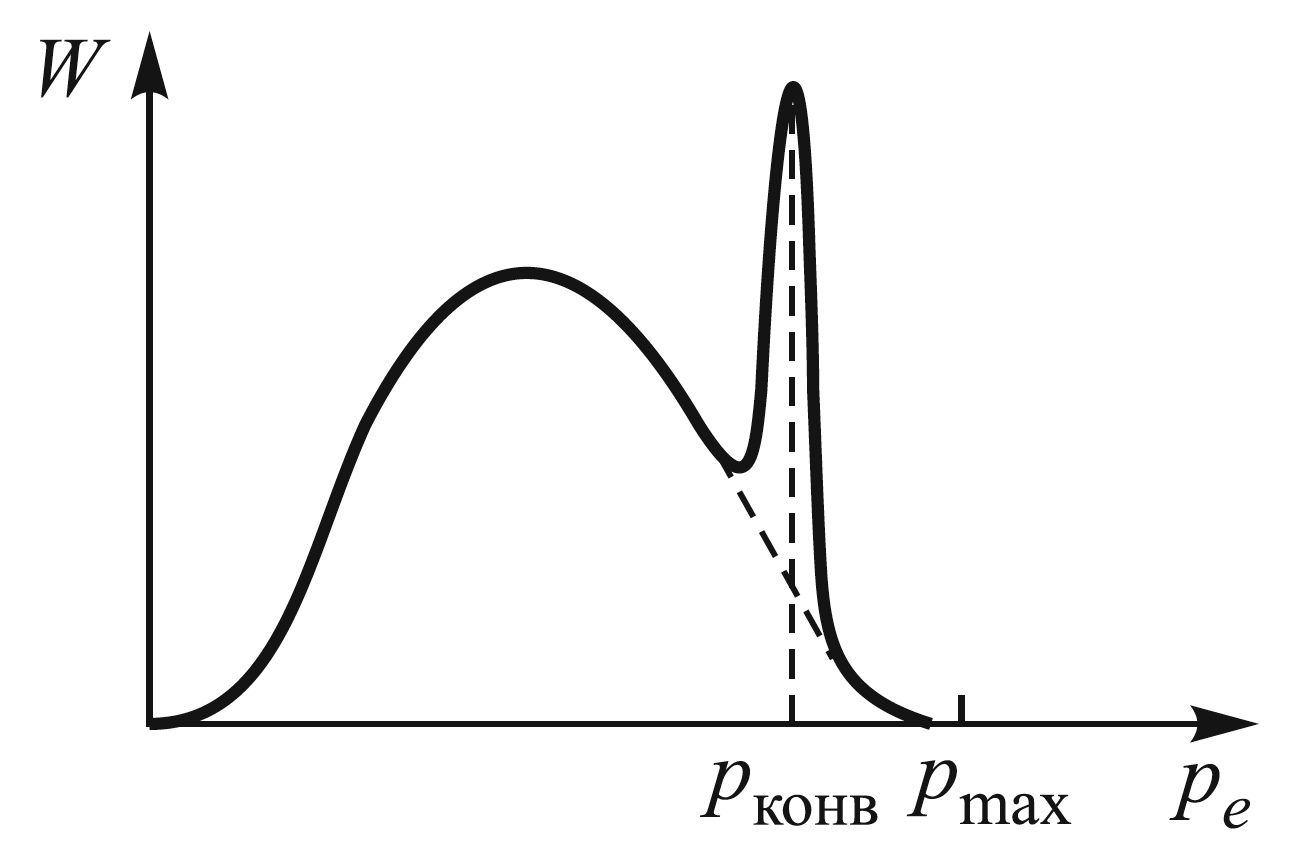
\includegraphics[scale=0.15]{Спектр.PNG}
	\end{figure}
		
	Дочерние ядра,  возникающие в результате $\beta$ - распада,  нередко оказываются возбуждёнными.  Возбуждённые ядра отдают свою энергию либо излучая гамма-квант, либо передавая избыток энергии одному из электронов с внутренних оболочек атома. Такие электроны имеют строго определённую энергию и называются конверсионными. Ширина монохроматической линии,  соответствующая конверсионным электронам,  определяет разрешающую силу спектрометра. \\
		
\textbf{Экспериментальная установка:}\\\par

\begin{figure}[h]
	\begin{center}
		\begin{minipage}[h]{0.48\linewidth}
			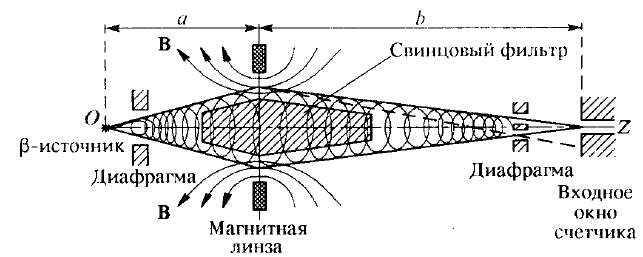
\includegraphics[width=1\linewidth]{Схема.PNG}
		\end{minipage}
	\hfill 
		\begin{minipage}[h]{0.48\linewidth}
			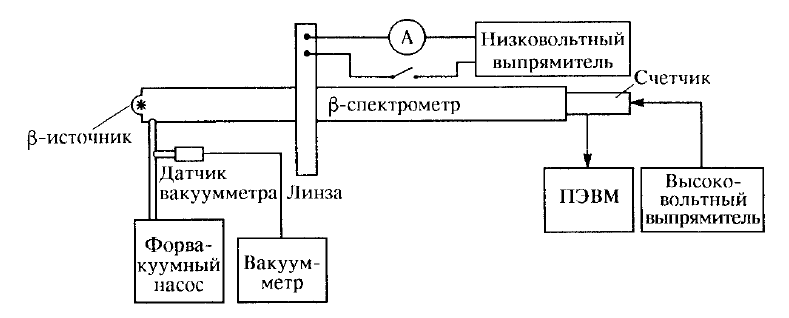
\includegraphics[width=1\linewidth]{Установка.PNG}
		\end{minipage}
	\end{center}
\end{figure}

	Радиоактивный источник $^{137}$Cs помещен внутрь откачанной трубы.  Электроны, сфокусированные магнитной линзой,  попадают в счетчик.  В газоразрядном счетчике они инициируют газовый разряд и тем самым приводят к появлению электрических импульсов на его электродах,  которые затем регистрируются пересчетным прибором.  В результате попадания электронов в сцинтиллятор на выходе фотоумножителя появляются электрические импульсы, которые заносятся в память персонального компьютера и выводятся на экран монитора.

	Энергию $\beta$-частиц определяют с помощью $\beta$ - спектрометров.  В работе используется магнитный спектрометр с <<короткой линзой>>.  Электроны,  испускаемые радиоактивным источником,  попадают в магнитное поле катушки,  ось которой параллельна оси OZ.  Траектории электронов в магнитном поле представляют собой схематически показанные на рисунке сложные спирали,  сходящиеся за катушкой в фокусе,  расположенном на оси OZ.

	Как показывает расчет,  для заряженных частиц тонкая катушка эквивалентна линзе.  Ее фокусное расстояние $f$ зависит от импульса электронов $p_e$ и от силы тока $I$,  протекающего через катушку следующим образом:

\[\frac{1}{f} \propto \frac{I^2}{p_e^2}\]

	При заданной силе тока на входное окно счетчика фокусируются электроны с определенным импульсом.  При изменении тока в катушке на счетчик последовательно фокусируются электроны с разными импульсами.  Так как геометрия прибора в течение всего опыта остается неизменной, импульс сфокусированных электронов пропорционален величине тока $I$:

\[p_e = kI,  \]
где $k$ -- константа прибора,  которая определяется по какой-нибудь известной конверсионной линии.

Величина $\Delta p_e$ -- ширина интервала импульсов,  регистрируемых при заданном значении тока,  называется разрешающей способностью $\beta$ - спектрометра.  Рассмотрим теперь связь между числом частиц,  регистрируемых установкой,  и функций $W(p_e) = dN/dp_e$:

\[N(p_e) \simeq W(p_e) \Delta p_e\]

Найдем $\Delta p_e$:

\[\Delta p_e = \dfrac{1}{2} \dfrac{\Delta f}{f} p_e\]

Таким образом,  ширина интервала $\Delta p_e$,  регистрируемого спектрометром,  пропорциональна величине импульса.  Получим окончательно:

\[N(p_e) = CW(p_e)p_e, \]
где $C$ -- некоторая константа.\\

\textbf{Ход работы:}\\\par

\begin{enumerate}

	\item Откачаем воздух из полости спектрометра,  включим ПЭВ,  включим формирователь импульсов и питание магнитной линзы.
	
	\item Проведем измерение $\beta$ - спектра,  изменяя ток в магнитной линзе от нуля до максимального значения через 0,2 А. При каждом значении тока будем измерять частоту попадания частиц в детектор за 80 секунд.
	
\newpage

	\begin{figure}[h!]
	    \centering
		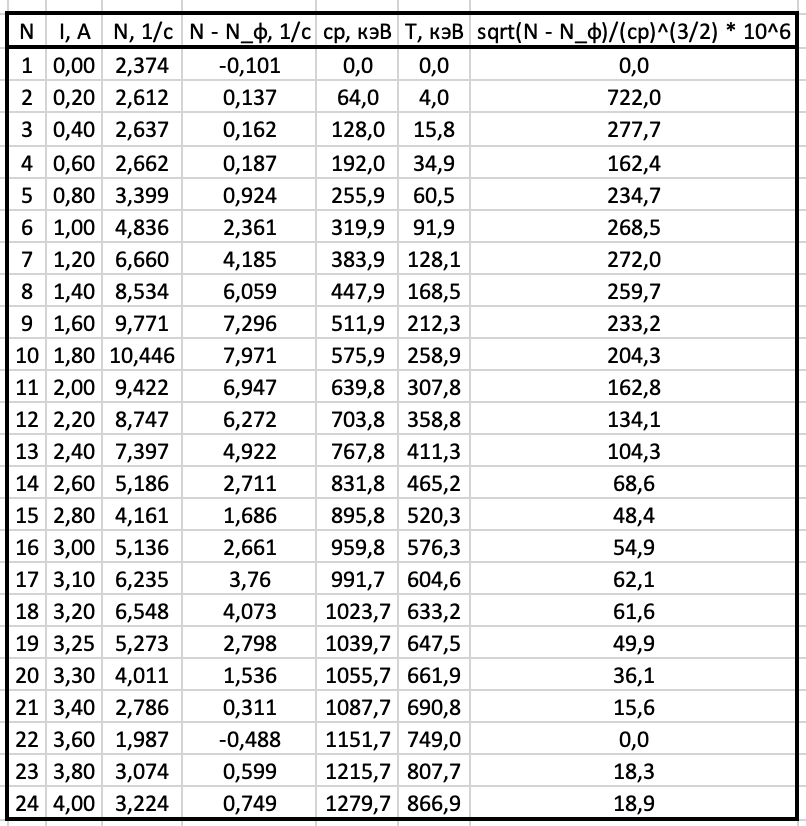
\includegraphics[scale=0.9]{Таблица_1.PNG}
	\end{figure}	

	Спектр частиц:

	\begin{figure}[h!]
	    \centering
		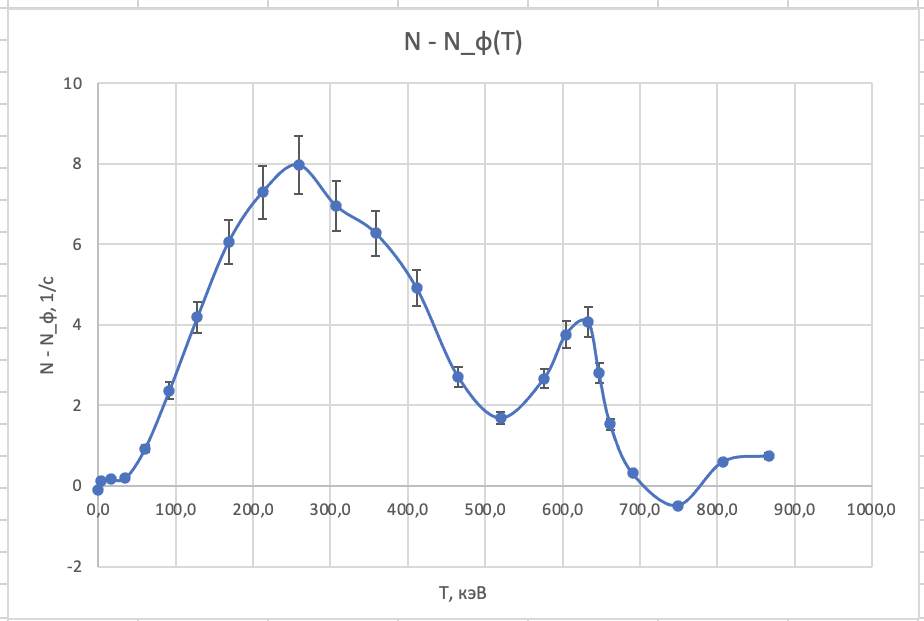
\includegraphics[scale=0.9]{График_1.PNG}
	\end{figure}	

	\item Измерим фон:
	
	\begin{figure}[h!]
	    \centering
		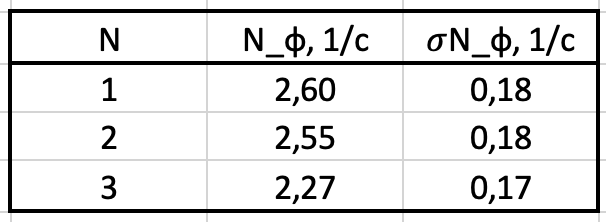
\includegraphics[scale=0.7]{Таблица_2.PNG}
	\end{figure}
	
	\[N_\text{ф} = (2,47 \pm 0,10) \text{ с}^{-1}\]

	\item Прокалибруем спектрометр,  с учетом того,  что $T = 634$кэВ,  $cp_\text{к} = 1013, 5$ кэВ.  Значение тока,  при котором достигается конверсионный пик: $I_\text{к} \approx 3,2$ А.  Тогда:
	
	\[ck = \frac{cp_\text{к}}{I_\text{к}} \approx 316,7 \text{ кэВ/А}\]

	\item Число электронов с импульсами,  лежащими в интервале $p$ до $p + dp$,  может быть записано как:
	
	\[N(p) dp \approx (cp)^3 (E_e - E)^2 dp \]

	Или

	\[\frac{\sqrt{N(p)}}{(cp)^{3/2}} \approx E_e - E \]

	Построим график Ферми - Кюри:

	\begin{figure}[h!]
	    \centering
		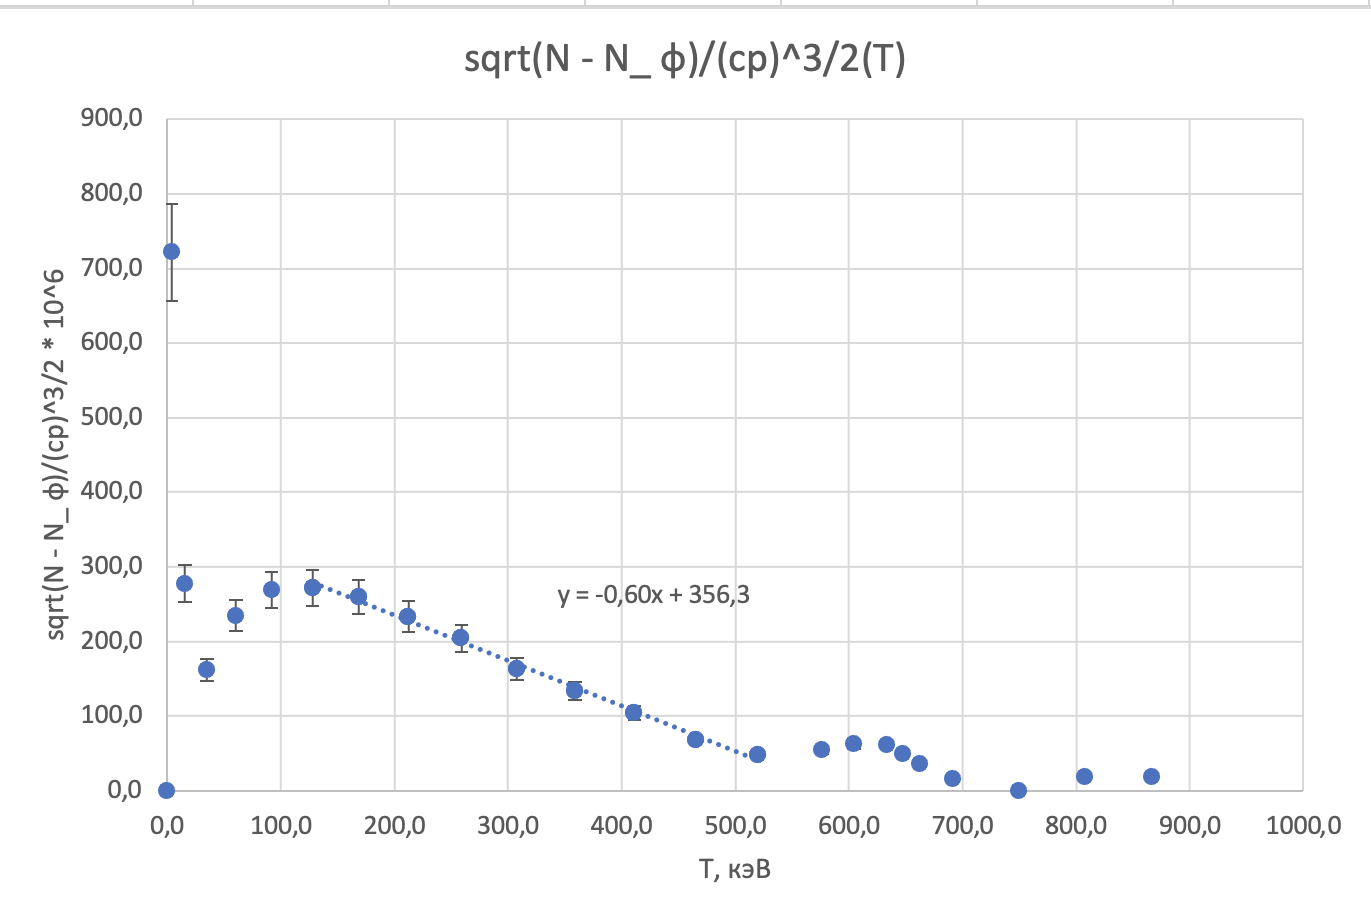
\includegraphics[scale=0.6]{График_2.PNG}
	\end{figure}

	Тогда получаем:
	
	\[E_e = (594 \pm 22) \text{кэВ}\]

\end{enumerate}

\textbf{Вывод:}\\\par

	В результате выполнения лабораторной работы был изучен энергетический спектр $\beta$ - частиц при распаде ядер $^{137}$Cs.  
	
	Мы экспериментально удостоверились в том,  что спектр $\beta$ - частиц имеет вид широкого купола,  причем данная кривая плавно касается оси абсцисс в области максимальной энергии электронов $E_e$. Также в спектре отчетливо наблюдается конверсионный пик.
	
	Было определено значение максимальной энергии $E_e$:
	
	\[E_e = (594 \pm 22) \text{ кэВ}\]
	
	\[E_{e\text{ табл}} = 512 \text{ кэВ}\]
	
	 Экспериментальное значение достаточно хорошо согласуется с табличным.

\end{document}